\documentclass[a4paper, 12pt]{report}
\usepackage{cmap}
\usepackage{amssymb}
\usepackage{amsmath}
\usepackage{graphicx}
\usepackage{amsthm}
\usepackage{upgreek}
\usepackage{setspace}
\usepackage{mathtools}
\setcounter{secnumdepth}{5}
\setcounter{tocdepth}{5}
\numberwithin{equation}{section}
\renewcommand{\theequation}{\arabic{equation}}
\usepackage[T2A]{fontenc}
\usepackage[utf8]{inputenc}
\usepackage[normalem]{ulem}
\usepackage{mathtext} % русские буквы в формулах
\usepackage[left=2cm,right=2cm, top=2cm,bottom=2cm,bindingoffset=0cm]{geometry}
\usepackage[english,russian]{babel}
\usepackage[unicode]{hyperref}
\newenvironment{Proof} % имя окружения
{\par\noindent{$\blacklozenge$}} % команды для \begin
{\hfill$\scriptstyle\square$}
\newcommand{\Rm}{\mathbb{R}}
\newcommand{\Cm}{\mathbb{C}}
\newcommand{\Z}{\mathbb{Z}}
\newcommand{\I}{\mathbb{I}}
\newcommand{\N}{\mathbb{N}}
\newcommand{\rank}{\operatorname{rank}}
\newcommand{\Ra}{\Rightarrow}
\newcommand{\ra}{\rightarrow}
\newcommand{\FI}{\Phi}
\newcommand{\Sp}{\text{Sp}}
\newcommand{\ol}{\overline}

\renewcommand{\leq}{\leqslant}
\renewcommand{\geq}{\geqslant}

\renewcommand{\alpha}{\upalpha}
\renewcommand{\beta}{\upbeta}
\renewcommand{\gamma}{\upgamma}
\renewcommand{\delta}{\updelta}
\renewcommand{\varphi}{\upvarphi}
\renewcommand{\phi}{\upvarphi}
\renewcommand{\tau}{\uptau}
\renewcommand{\theta}{\uptheta}
\renewcommand{\eta}{\upeta}
\renewcommand{\lambda}{\uplambda}
\renewcommand{\sigma}{\upsigma}
\renewcommand{\psi}{\uppsi}
\renewcommand{\mu}{\upmu}
\renewcommand{\omega}{\upomega}
\renewcommand{\xi}{\upxi}
\renewcommand{\epsilon}{\upvarepsilon}
\renewcommand{\rho}{\uprho}
\renewcommand{\varepsilon}{\upvarepsilon}

\renewcommand{\d}{\partial}
\renewcommand{\Re}{\operatorname{Re}}
\newcommand{\const}{\operatorname{const}}
\newcommand{\intx}{\int\limits_{x_0}^x}
\newcommand\Norm[1]{\left\| #1 \right\|}
\newcommand{\sumk}{\sum\limits_{k=0}^\infty}
\newcommand{\sumi}{\sum\limits_{i=0}^\infty}
\newtheorem*{theorem}{Теорема}
\newtheorem*{cor}{Следствие}
\newtheorem*{lem}{Лемма}
\title{\textbf{\Huge{Численные методы математической физики}}\\Конспект по 4 курсу 
	специальности «прикладная математика»\\(лектор А. М. Будник)}
\date{}
\begin{document}
	\maketitle
	\tableofcontents{}
	\newpage
	\section*{Введение.}
	В данном курсе мы будем рассматривать задачи математической физики в частных производных. Основной принцип решения состоит в том, что дифференциальное уравнение мы заменяем разностным и ищем приближенное решение на сетке узлов. Такой способ называется \textit{методом конечных разностей} (\textit{методом сеток}). А раздел численных методов, посвященный теории метода конечных разностей, носит название \textit{теория разностных схем}. 
	\\\\
	Выделим два основных момента при решении:
	\begin{enumerate}
		\item построение дискретных разностных аппроксимаций для уравнений математической физики и исследование основных характеристик этих аппроксимаций: погрешности, устойчивости и точности разностных схем;
		\item решение разностных уравнений прямыми или итерационными методами, которые выбираются из соображений экономичности вычислительного алгоритма.
	\end{enumerate}
	\chapter{Способы построения и исследования разностных схем.}
	\section{Сетки и сеточные функции.}
	При численном решении той или иной математической задачи мы не можем воспроизвести приближенное решение для всех значений аргумента. Поэтому в области задания функции выбирается конечное множество точек, и приближенное решение задачи ищется в этих точках.
	\\\\
	$\bullet$ \textit{Это множество называется \textbf{сеткой}, а отдельные точки этого множества -- \textbf{узлами сетки}.}
	\\\\
	$\bullet$ \textit{Функция, определенная в узлах сетки, называется \textbf{сеточной функцией}.}
	\\\\
	Заменяя области непрерывного изменения аргумента сеткой, то есть областью дискретного изменения аргумента, мы осуществляем аппроксимацию пространства решения дифференциального уравнения пространством сеточной функции.
	\\\\
	\textbf{Пример сетки на отрезке (одномерный случай).}\\\\
	В качестве области определения искомой функции мы рассматриваем отрезок на оси $x$.
	\begin{enumerate}
		\item \textbf{Равномерная сетка.}
		Не ограничивая общности, возьмем отрезок $[0,1]$ и разобьем его на $N$ равных частей точками $$x_0=0,\ x_1,\ \ldots,\ x_{N-1},\ x_N=1.$$
		Расстояние между соседними точками назовем \textit{шагом сетки} и обозначим его через $h$, а точки $x_i$ примем в качестве \textit{узлов сетки}, $i=\overline{0,N}$. Тогда множество всех $x_i$ составляют \textit{равномерную сетку} на отрезке $[0,1]$, которую будем обозначать следующим образом
		$$\overline \omega _ h = \left\{x_i = ih,\ i=\overline{0, N},\ h = \dfrac1N\right\}.$$
		\textit{Множество граничных узлов} обозначим как $$\gamma_h = \{x_0, x_N\}.$$
		А все остальные точки образуют \textit{множество внутренних узлов}
		$$ \omega _ h = \left\{x_i = ih,\ i=\overline{1, N-1},\ h = \dfrac1N\right\}.$$
		Таким образом, можно записать 
		$$\overline \omega _h = \omega _h \cup \gamma _h.$$
		\item \textbf{Неравномерная сетка.}
		Возьмем отрезок $[0,1]$ и разобьем его на $N$ частей точками $$0=x_0 < x_1 <\ldots< x_{N-1} < x_N=1.$$
		Тогда мы можем записать неравномерную сетку с граничными узлами 
		$$\hat {\overline \omega} _ h = \left\{x_i,\ i=\overline{0, N},\ x_0 = 0, \ x_N=1\right\}.$$
		Шаг неравномерной сетки зависит от номера узла и удовлетворяет условию нормировки $$\sum_{i=1}^{N} h_i=1,\ \text{где } h_i=x_i - x_{i-1}.$$
		Аналогично случаю равномерной сетки можно записать $$\hat {\overline \omega} _ h = \hat \omega_h \cup \hat\gamma _h.$$
	\end{enumerate}
	\textbf{Пример сетки на плоскости (двумерный случай).}
	\begin{enumerate}
		\item \textbf{Прямоугольник.} Исходная область прямоугольника $$\overline G = \{(x_1, x_2),\ 0\leq x_\alpha \leq l_\alpha,\ \alpha=1,2\}$$
		$$
	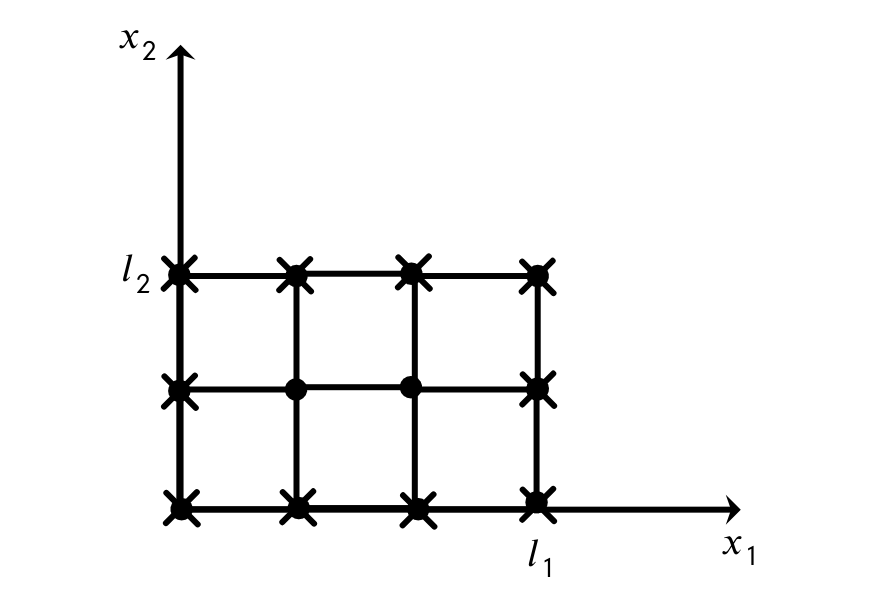
\includegraphics[scale=0.5]{images/img_1}
		$$
		(кружочками обозначены внутренние узлы, а крестиками -- внешние).\\\\
		Сначала построим равномерную сетку. Разобьем отрезки $[0, l_\alpha]$ на $N_\alpha$ частей точками $$0 = x_{\alpha,0} < x_{\alpha, 1} < \ldots < x_{\alpha, N_\alpha -1} < x_{\alpha, N_\alpha} = l_\alpha.$$ Через точки деления проводим прямые, параллельные координатной оси. В качестве узлов двумерной сетки возьмем точки пересечения этих прямых. Общее количество узлов сетки равно $(N_1+1) \times (N_2 + 1)$, а их распределение характеризуется векторным параметром $$h = \{h_{\alpha,1},\ldots, h_{\alpha, N_\alpha},\ h_{\alpha, i_\alpha} = x_{\alpha, i_\alpha} - x_{\alpha, i_\alpha-1},\ i_\alpha = \overline{1, N_\alpha}, \alpha=1,2\}.$$
		Тогда \textit{неравномерную двумерную сетку} можно обозначить
		$$\hat{ \overline \omega} _ h = \hat{ \overline \omega}_{h_1, h_2} = \hat{ \overline \omega} _ {h_1} \times \hat{ \overline \omega} _ {h_2} = \{(x_{1,i_1}, x_{2, i_2}),\ i_\alpha = \overline{0, N_\alpha},\ x_{\alpha, 0} = 0, x_{\alpha, N_\alpha } = l_\alpha,\ \alpha=1,2\}.$$
		Если по каждому направлению шаги сетки равны между собой, то мы получим \textit{двумерную равномерную сетку}
		$${ \overline \omega} _ h = { \overline \omega}_{h_1, h_2} = \hat{ \overline \omega} _ {h_1} \times \hat{ \overline \omega} _ {h_2} = \left\{(x_{1,i_1}, x_{2, i_2}),\ x_{\alpha, i_\alpha} = i_\alpha h_\alpha,\ i = \overline{0, N_\alpha},\ h_\alpha=\frac{l_\alpha}{N_\alpha},\ \alpha=1,2\right\}.$$
		\item \textbf{Область сложной формы.} Пусть нам дана область нерегулярной (сложной) формы $\overline G = G \cup \Gamma$. Для построения сетки мы заключим эту область в прямоугольник $[a,b]\times [c,d]$. В этом прямоугольнике мы строим прямоугольную сетку. Для простоты зададим прямоугольную равномерную сетку. 
		$$
			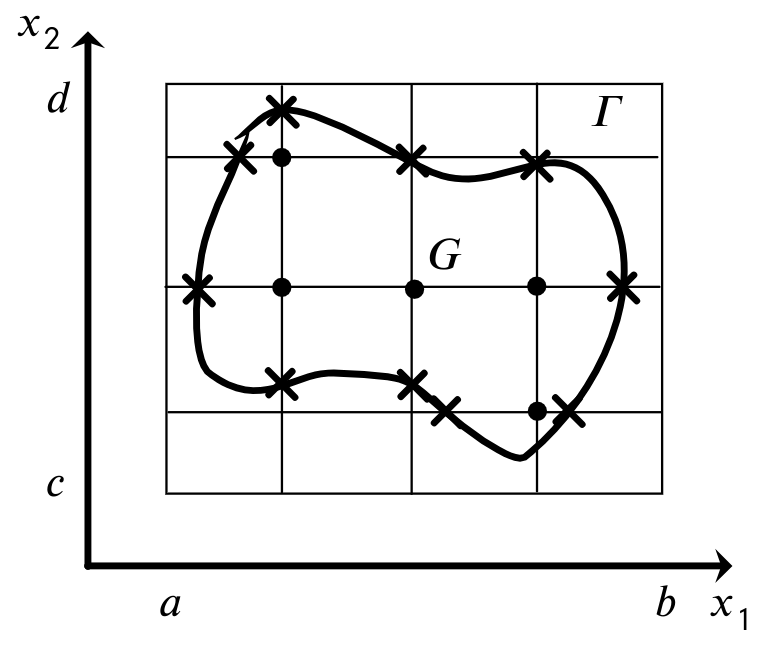
\includegraphics[scale=0.5]{images/img_2}
		$$
		Те узлы, которые попали внутрь этой сетки, будем считать \textit{внутренними}, обозначим их совокупность $\omega _h$. Точки пересечения прямых $x_\alpha = i_\alpha l_\alpha$, $\alpha=1,2$ с границей $\Gamma$ назовем \textit{граничными узлами}, обозначим их совокупность $\gamma_h$. Тогда сеткой будет множество узлов $$\overline \omega_h = \omega_h \cup \gamma_h$$
		Если исходная сетка в прямоугольнике $[a,b]\times [c,d]$ является равномерной, то сетка $\overline\omega_h$ в области $\overline G$ является неравномерной.\\\\
	\end{enumerate}
	\textbf{Замечания.}
	\begin{enumerate}
		\item Аналогичным образом строятся сетки и большей размерности. 
		\item В зависимости от геометрии исходной области можно использовать и другие ортогональные системы координат.
		\item Кроме прямоугольных сеток можно строить, так называемые, треугольные сетки, элементарными ячейками которой являются треугольники. 
	\end{enumerate}
	Пусть $u(x)$ --- это функция непрерывного аргумента $x = (x_1, \ldots, x_p)\in \overline G$ и $u(x) \in H_0$ ($H_0$ --- функциональное пространство). Если в области $\overline G$ введена сетка $\overline \omega_h$, то вместо функции $u(x)$ можно рассматривать функцию дискретного аргумента $y(x) = y_h$, где $x\in \ol \omega _h$, и эту функцию будем называть \textit{сеточной функцией}, значения которой вычисляются в узлах, а сама функция зависит от шага сетки $h$.\\\\
	Множество сеточных функций образует пространство $H_h$ -- \textit{пространство сеточных функций}. Следуя методу конечных разностей, мы заменяем пространство $H_0$ пространством $H_h$. Если $h$ -- параметр, то мы можем рассматривать множество сеточных пространств $\{H_h\}$ для каждого фиксированного $h$.\\\\
	Для того, чтобы оперировать функций, нам нужен аппарат для исследования функций и их сравнения. Мы рассматриваем линейные пространства, а для линейных пространств вводится понятие нормы. Соответственно мы определяем \textit{сеточный аналог нормы} $$\Norm {\cdot}_0 \sim \Norm {\cdot} _h.$$
	Например, если $H_ 0 = C[0,1]$, то в нем вводится норма $\Norm {\cdot}_0 = \underset{x\in [0,1]} {\max}|u(x)|$. Тогда сеточным аналогом может быть норма $$\Norm {\cdot}_h = \underset{x \in \ol \omega_h}{\max}|y(x)|.$$
	Если взять $H_ 0 = L_2[0,1]$, то в нем вводится норма $\Norm {\cdot}_0 = (u,u)^\frac12$. Тогда сеточным аналогом может быть норма $$\Norm {\cdot}_h = \left(\sum_{i=1}^{N-1}hy_i^2\right)^\frac12.$$
	Предположим, что функция $u(x)$ -- это решение некоторой дифференциальной задачи. Тогда $y_h(x)$ -- это решение приближенной, или разностной задачи. Для сравнения точного и приближенного решений сеточная функция доопределяется во всех точках области $\ol G$. В результате получается функция непрерывного аргумента $\widetilde{y}_h$, тогда точность решения может быть оценена как $$\Norm{\widetilde{y}_h - u}_0.$$
	Другой подход заключается в том, что мы исходное пространство $H_0$ отображаем в пространство $H_h$. Каждой функции $u(x)\in H_0$ ставится в соответствие сеточная функция $u_h(x), x \in \ol \omega _h$, при этом $u_h = P_h u \in H_h$, где $P_h$ -- это линейный оператор проектирования из $H_0$ в $H_h$. Тогда точность решения оценивается как $$\Norm{y-u_h}_h.$$ Для того, чтобы эта операция была корректна, естественно требовать, чтобы норма пространства $H_h$ аппроксимировала норму пространства $H_0$, то есть $$\lim\limits_{h\to 0}\Norm{u_h}_h = \Norm{u}_0.$$
	$\bullet$ \textit{Это требование называется \textbf{условием согласованности норм}.}\\\\
	\section{Разностная аппроксимация дифференциальных операторов.}
	\subsection{Локальная аппроксимация.}
	Пусть задан линейный дифференциальный оператор $L$ действующий на функцию $u=u(x)$. Для того, чтобы аппроксимировать (приближенное вычислить) его в любой точке $x\in \omega _h$ разностным оператором $L_h$, необходимо в начале указать или выбрать шаблон $\text {Ш} (x)$. \\\\
	$\bullet$ \textit{Под \textbf{шаблоном} $\text{Ш}(x)$ мы понимаем множество узлов сетки, которое будет использоваться при аппроксимации оператора $L$ оператором $L_h$ в точке $x$.}\\\\
	$\bullet$ \textit{П\textbf{огрешность аппроксимации дифференциального оператора $L$ разностным оператором $L_h$ в точке $x$} называется величина }
	\begin{equation}
		\psi(x) = L_hu(x) - Lu(x),\ x\in \omega_h.
	\end{equation}
	$\bullet$ \textit{Будем говорить, что \textbf{разностный оператор $L_h$ аппроксимирует дифференциальный оператор $L$ с порядком $m>0$ в точке $x$}, если можно представить} $$\psi(x) = O(h^m).$$
	Рассмотрим способ построения разностных операторов, получивший название \textit{метод неопределенных коэффициентов}. На выбранном шаблоне $\text{Ш}(x)$ разностную аппроксимацию будем искать в виде линейной комбинации значений функции в точках шаблона \begin{equation}
		L_hu(x) = \sum_{\xi \in \text{Ш}(x)} A_h(x, \xi) u(\xi).
	\end{equation}
	В формуле (2) $A_h(x, \xi)$ -- это неизвестные коэффициенты, выбранные таким образом, чтобы погрешность аппроксимации имела в точке $x$ заданный (чаще всего максимально возможный) порядок. Практический выбор значений коэффициентов осуществляется путем разложения погрешности аппроксимации в ряд Тейлора, то есть мы представляем $$\psi(x) = \sum_{\xi \in \text{Ш}(x)} A_h(x, \xi) u(\xi) - Lu(x),$$
	а затем раскладываем получившееся выражение в ряд Тейлора в окрестности точки $x$. После приведения мы получаем в итоге линейную комбинацию 
	$$\psi(x) = \sum_{\xi \in \text{Ш}(x)} A_h(x, \xi) u(\xi) - Lu(x) = \sum_{|j|\geq 0} B_h^{(j)}(x) u^{(j)}(x).$$
	После этого мы приравниваем к нулю максимально возможное количество первых членов этого разложения. Как правило, количество этих членов совпадает с количеством неизвестных коэффициентов. После этого, решив систему линейных уравнений, находим коэффициенты $A_h$ и по формуле (2) записываем искомый разностный оператор $L_h$.
	\\\\
	\textbf{Замечания.}
	\begin{enumerate}
		\item Выбор шаблона зависит от порядка производных, входящих в исходный операторов $L$, а также от требуемой точности аппроксимации.
		\item Легко видеть, что для аппроксимации дифференциального оператора, содержащего производную $k$-ого порядка по некоторой переменной, необходимо использовать шаблон, содержащий не менее $(k+1)$ точку вдоль координатного направления соответствующей переменной.
		\item Метод неопределенных коэффициентов является не единственным способом построения разностных операторов. Известен в литературе также метод \textit{численного дифференцирования}.
	\end{enumerate}
	\textbf{Примеры.}
	\begin{enumerate}
		\item Пусть задан дифференциальный оператор $$Lu(x) = \dfrac{d u(x)}{dx} = u'(x).$$
		\begin{enumerate}
			\item Пусть нам дан шаблон $\text{Ш}(x) = \{x, x+h\}$. Тогда по формуле (2) составляем линейную комбинацию
			$$u(x) = a_0 u(x) + a_1u(x+h).$$
			Записываем выражение для погрешности аппроксимации
			$$\psi(x) a_0u(x) + a_1u(x+h) - u'(x).$$
			Затем производим разложение выражения в ряд Тейлора в окрестности точки $x$ и приводим подобные при значениях функции и ее производных
			$$\psi(x) a_0u(x) + a_1u(x+h) - u'(x) = \underbrace{(a_0+a_1)}_{B ^{(0)}}u(x) + \underbrace{(ha_1 - 1)}_{B^{(1)}} u'(x) + \dfrac{h^2}{2} a_1 u''(x) + \ldots.$$
			Приравнивая коэффициенты $B^{(j)}$ к нулю, получаем систему линейных уравнений 
			$$\begin{cases}
				a_0+a_1 = 0,\\
				ha_1 - 1= 0.
			\end{cases}$$
			Тогда $$a_0 = -\dfrac 1h,\ a_1 = \dfrac 1h.$$
			Таким образом, мы построили разностный оператор вида 
			\begin{equation}
				L_hu(x) = \dfrac{u(x+h) - u(x)}{h} = u_x
			\end{equation}
			$\bullet$ \textit{Обозначение называется \textbf{правой разностной производной}.}\\\\
			При этом $$\psi(x) = \dfrac h2 u''(x) + \ldots = O(h),$$ то есть разностный оператор (3) аппроксимирует исходный оператор $L$ с первым порядком.\\\\
			$\bullet$ \textit{Величина $\dfrac h 2 u''(x)$ называется \textbf{главным членом погрешности аппроксимации}.}
			\item Пусть нам дан шаблон $\text{Ш}(x) = \{x-h, x\}$. Поступая аналогичным образом, мы можем построить оператор вида 
			\begin{equation}
				L_hu(x) = \dfrac{u(x) - u(x-h)}{h} = u_{\ol x}
			\end{equation}
			$\bullet$ \textit{Обозначение $u_{\ol x}$ называется \textbf{левой разностной производной}. }
			\\\\
			Легко видеть, что $$\psi(x) = -\dfrac h2 u''(x) + \ldots = O(h).$$ 
			\item Пусть нам дан шаблон $\text{Ш}(x) = \{x-h, x, x+h\}$. Проделав те же вычисления, мы получим выражение 
			\begin{equation}
				L_hu(x) = \dfrac{u(x+h) - u(x-h)}{2h} = u_{\circ x}
			\end{equation}
			$\bullet$ \textit{Обозначение $u_{\ol x}$ называется \textbf{центральной разностной производной}.}
			\\\\
			Легко видеть, что $$\psi(x) = -\dfrac {h^2}{6} u'''(x) + O(h^4) = O(h^2).$$ 
		\end{enumerate}
		Можно заметить, что с увеличением точек шаблона будет также увеличиваться погрешность аппроксимации.\\\\
		Можно построить однопараметрическое семейство операторов для аппроксимаиции первой производной следующего вида $$L_h^{(\sigma)}u(x) = \sigma u_x + (1-\sigma)u_{\ol x},$$
		где $\sigma$ -- это любое вещественное число. Выражение для погрешности имеет следующий вид
		$$\psi(x) = (2\sigma - 1)\dfrac h2 u''(x) + O(h^2).$$
		Очевидно, что при любом $\sigma \ne \frac 12$ разностный оператор будет иметь первый порядок аппроксимации $\psi(x) = O(h).$ Иначе мы получаем второй порядок аппроксимации $\psi(x) = O(h^2)$ , при этом легко видеть, что $$L_h^{(0,5)} = \dfrac 12(u_x + u_{\ol x}) = u_{\hat x}.$$
		\item Пусть нам дан дифференциальный оператор $$Lu(x) = u''(x).$$ Оператор второго порядка, поэтому для аппроксимации нужно как минимум 3 точки. Возьмем шаблон $\text{Ш}(x) = \{x-h, x, x+h\}$. Применяя метод неопределенных коэффициентов, мы получим следующий разностный оператор \begin{equation}
		L_h u(x) = \dfrac{u(x+h) - 2u(x) + u(x-h)}{h^2}=u_{\ol xx}
		\end{equation}
		$\bullet$ \textit{Обозначение $u_{\ol x x}$ называется \textbf{второй разностной производной}.}\\\\
		Погрешность будет иметь вид $$\psi(x) = \dfrac {h^2}{12} u^{IV}(x) + O(h^4) = O(h^2),$$ то есть имеет второй порядок, а не первый, как мы могли ожидать. Оказывается, что именно симметрия шаблона обеспечивает повышение порядка аппроксимации. Но на произвольной сетке мы получили бы первый порядок аппроксимации.\\\\
		\textbf{Замечания.}
		\begin{enumerate}
			\item Символы, используемые для обозначения разностных производных неслучайны, а является формальными операторами разностного дифференцирования и предписывают, как осуществлять аппроксимации. Например, если мы имеем разностный оператор $u_{\ol x x}$, то можно записать
			\begin{multline*}
				u_{\ol x x} = (u_{\ol x}(x))_x = \dfrac{u_{\ol x}(x+h) - u_{\ol x}(x)}{h} = \dfrac{1}{h}\left(\dfrac{u(x+h) - u(x)}{h} - \dfrac{u(x) - u(x-)}{h}\right) =\\= \dfrac{u(x+h) - 2u(x) - u(x-h)}{h^2}.
			\end{multline*}
			Можно также записывать $$u_{\ol x}(x+h) = u_x(x),\ \dfrac12 (u_x + u_{\ol x}) = u_{\circ x}.$$ Соответственно, мы можем конструировать разные операторы. Существуют также и разностные аналоги формул Грина.
			\item Разложение погрешности $\psi(x)$ по степеням $h$ можно использовать для повышения порядка аппроксимации. Например, мы можем заменить четвертую производную четвертой разностной производной в выражении $$u_{\ol x x}(x) - u''(x) = \dfrac{h^2}{12} u^{IV}(x) + O(h^4) = \dfrac{h^2}{12}\left(u_{\ol x x\ol x x}(x) + O(h^2)\right) + O(h^4).$$
			Тогда можно построить разностный оператор $$L_hu(x) = u_{\ol x x}(x) - \dfrac{h^2}{12} u_{\ol x x\ol x x}(x).$$
			Шаблон уже будет $$\text{Ш}(x) = \{x-2h, x-h, x, x+h, x+2h\},$$ а погрешность аппроксимации $$\psi(x) = O(h^4).$$
		\end{enumerate}
		\item Пусть дан дифференциальный оператор $$Lu = \dfrac{\d u}{\d t} - \dfrac{\d ^2 u}{\d x ^2},\ u=u(x,t),\ (x,t) \in \omega_{h\tau}.$$
		\begin{enumerate}
			\item Шаблон может иметь вид [рисунок три точки внизу, одна точка сверху. Центральная нижняя жирная].\\\\
			\item Шаблон может иметь вид [рисунок три точки сверху, одна точка снизу. Центральная нижняя жирная].\\\\
			\item Шаблон может иметь вид [рисунок три точки сверху, три точки снизу, центральная нижняя жирная].
		\end{enumerate}
		Для шаблона (а) мы можем записать оператор $$L_{h\tau} u = \dfrac{u(x, t+\tau) - u(x,t)}{\tau} - \dfrac{u(x+h, t) - 2u(x,t) + u(x-h, t)}{h^2}.$$
		Такая форма записи называется \textit{индексной.}
		Учитывая введенные обозначения, мы можем записать этот оператор также в форме 
		\begin{equation}
			L_{h\tau} u = \dfrac{u(x, t+\tau) - u(x,t)}{\tau} - \dfrac{u(x+h, t) - 2u(x,t) + u(x-h, t)}{h^2} = u_t - u_{\ol x x}.
		\end{equation}
		Используем следующие обозначения: $$u(x,t) = u,\ u(x, t+\tau) = \hat u, \ u(x, t-\tau) = \check {u}.$$
		Тогда для случая (b) можно записать \begin{equation}
			L_{h\tau} u = u_t - \hat u_{\ol x x}.
		\end{equation}
		Для случая (c) мы можем построить однопараметрическое семейство аппроксимаций вида
		\begin{equation}
			L_{h\tau}^{(\sigma)}u = u_{\hat t} - (\sigma \hat u_{\ol x x} - (1-\sigma) u_{\ol x x}),\ \sigma \ne 0,\ \sigma \ne 1.
		\end{equation}
		Разностный оператор (9) аппроксимирует исходный дифференциальный оператор со вторым порядком по $x$ при любых $\sigma$ и первым порядком по $\tau$ при $\sigma =0, \sigma = 1$. Или вторым порядком по $\tau$ при $\sigma = \dfrac 12$. То есть можно записать записать 
		\begin{equation}
			\begin{cases}
				\psi(x,t) = O(\tau + h^2),\ \sigma \ne \dfrac 12,\\
				\psi(x,t) = O(\tau^2 + h^2),\ \sigma = \dfrac 12.
			\end{cases}
		\end{equation}
		\item Пусть дан дифференциальный оператор $$Lu = \dfrac{\d ^2u}{\d t^2} - \dfrac{\d ^2 u}{\d x^2}.$$
		Сейчас по каждому из направлений у нас будет по 3 точки.
		\begin{enumerate}
			\item Шаблон может иметь вид [рисунок три точки внизу, две вверх по центру. Центральная жирная ].\\\\
			\item Шаблон может иметь вид [рисунок как предыдущий но наоборот].\\\\
			\item Шаблон может иметь вид [рисунок одна жирная по центру и по одной в каждом направлении].
			\item Шаблон может иметь вид [4 квадрата, жирная по центру].
		\end{enumerate}
		Запишем двухпараметрическое семейство для варианта (d)
		\begin{equation}
			L_{h\tau}^{(\sigma_1, \sigma_2)}u = u_{\ol t t} - (\sigma_1 \hat u_{\ol x x} + (1-\sigma_1 - \sigma _2) u_{\ol x x} + \sigma_2 \check u_{\ol x x}).
		\end{equation}
		Для шаблона (а) \begin{equation}
			L_{h\tau}^{(0,1)} u= u_{\ol t t} - \check u_{\ol x x}.
		\end{equation}
		Для шаблона (b) \begin{equation}
			L_{h\tau}^{(1,0)} u= u_{\ol t t} - \hat u_{\ol x x}.
		\end{equation}
		Для шаблона (c) \begin{equation}
			L_{h\tau}^{(0,0)} = u_{\ol t t} - u_{\ol x x}.
		\end{equation}
			\end{enumerate}
		Погрешность аппроксимации оператора (14) будет равна $$\psi(x,t) = O(h^2 + \tau^2),\ \sigma_1=\sigma_2 = 0.$$
		Если же $\sigma_1 = \sigma_2 = \sigma$, то погрешность будет также иметь второй порядок
		$$\psi(x,t) = O(h^2 + \tau^2).$$
		Для других значений погрешность аппроксимации по $h$ понижается.
	\end{document}
	


	